Giving the customer the possibility to participate in the development of a
product by providing him transparency regarding the overall progress and by 
implementing its feedback is one of the most important success factors.
Especially if the final results of the collaboration are not explicitly clear or
if the project is some kind of research work, it is of highest importance to
gather the customer's feedback continuously. The gained feedback serves as an
input in adapting the product or even the whole process of development.

\begin{figure}
\centering
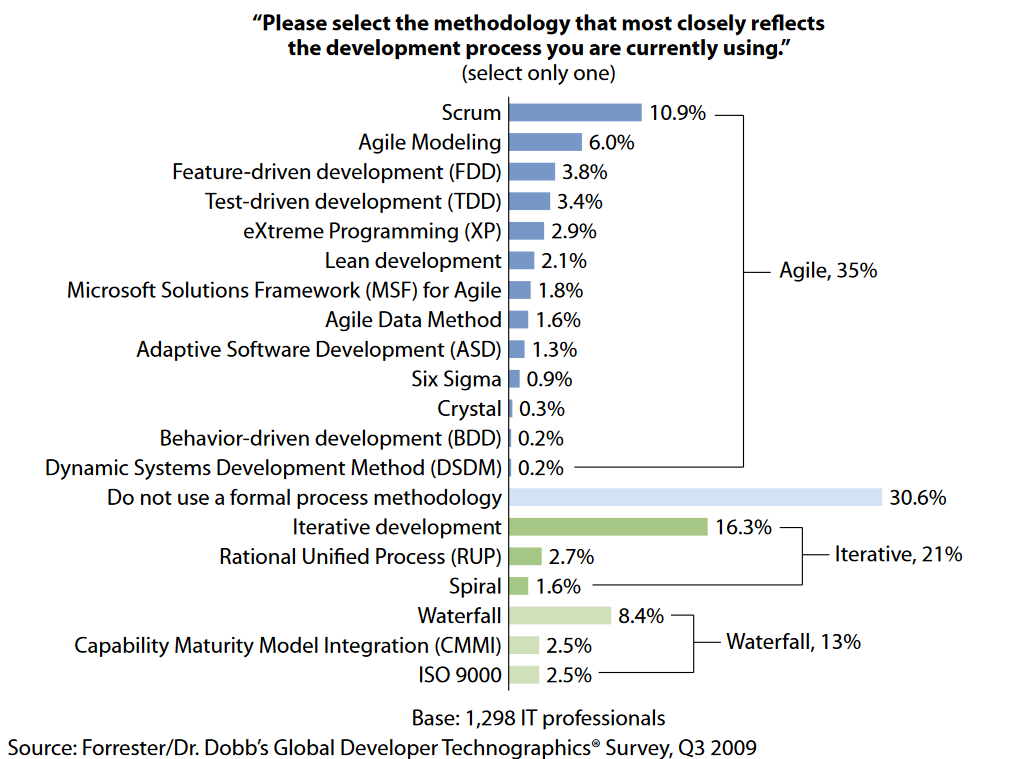
\includegraphics[width=0.75\textwidth]{res/customerVoice/applicationOfAgileMethods.PNG}
\caption{Adoption of agile Methods in Software Development (\cite{forrester})}
\label{fig:agileAdoption}
\end{figure}

Especially in the area of software development, the need for constant
interaction between a manufacturer and its customer is widely acknowledged. This
fact can be demonstrated by the adoption of agile methods (see figure
\ref{fig:agileAdoption}). These methods, like XP, Scrum and FDD, offer the
possibility of high transparency, short feedback-cycles and increased
flexibility regarding changes in the requirements or in the market -�
characteristics that proved themselves good and that are strongly wanted 
by the manufacturers adopting agile methods (see figure
\ref{fig:agileFeatures}).

\begin{figure}
\centering
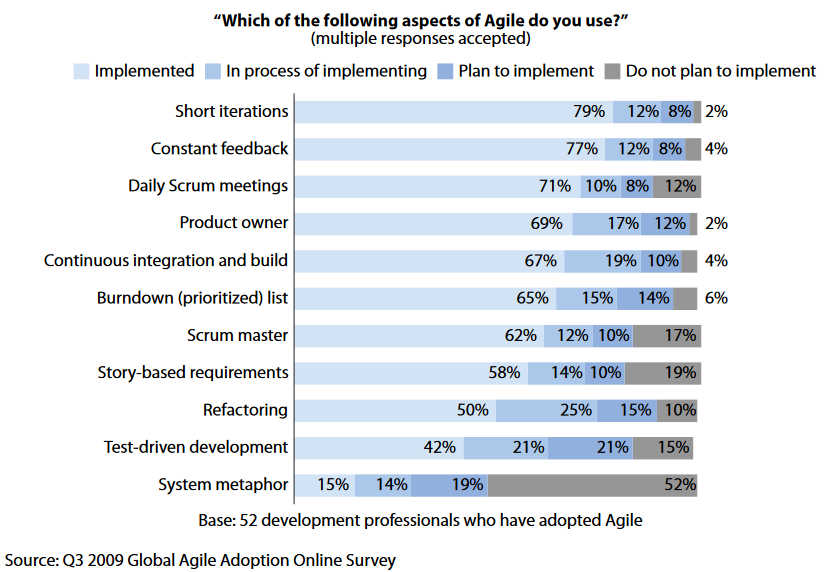
\includegraphics[width=0.75\textwidth]{res/customerVoice/aspectsOfAgile.PNG}
\caption{Adoption of agile Methods in Software Development (\cite{forrester})}
\label{fig:agileFeatures}
\end{figure}

\section{Determining the Modalities of Collaboration}
\label{sect:firstQuestionnaire}
To embed a process that as well satisfies the customer as it provides the
manufacturer the possibility to get as much useful input and feedback as
possible, the modalities of collaboration are negotiated as a first step. The
salient points in this negotiation are:

\begin{itemize}
\item{Who is the customer's specialist contact person and how should the
communication with him/her take place?}
\item{Who is the customer's technical contact person and how should the
communication with him/her take place?}
\item{In which way will the customer contact our company if necessary?}
\item{What are the customers preferences regarding the reports on the project's progress?}
\end{itemize}

While some of these points like the contact information of a certain person in
charge are only of informational kind, other points like the desired way of
communication are of high importance. Since there are certain preferences in our
company regarding the length of the iterations and the way how the communication
should take place, the CORE value of the customer's answers in respect of our
company's preferences is calculated.

\subsection{Results}
The results of the first questionnaire that serves to determine the modalities
of collaboration between our company and our customer are presented in this
section. The analysis of the results can be found in section
\ref{sect:q1_results}. Answers that contain personal data like contact
information are omitted.

\begin{figure}
\centering
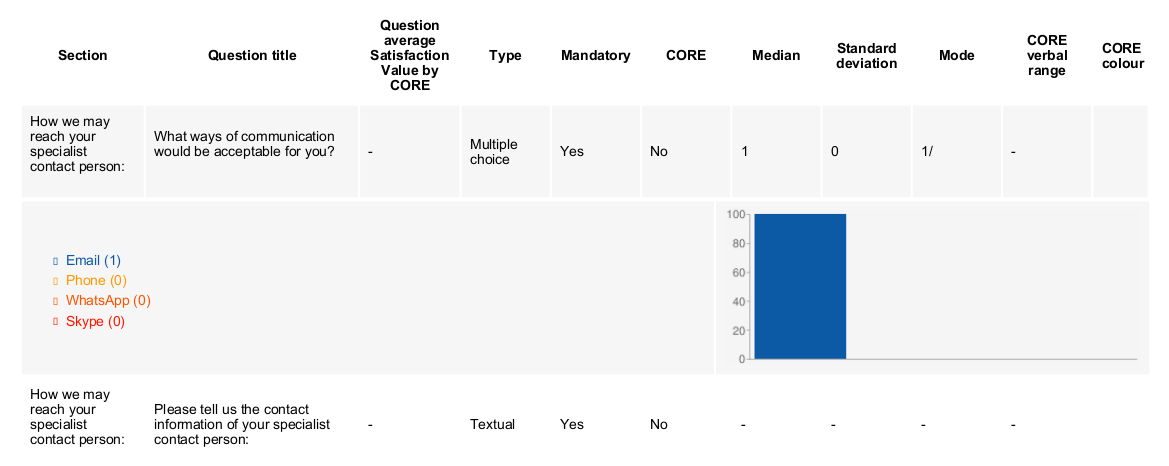
\includegraphics[width=\textwidth]{res/customerVoice/q1_results/q1.png}
%\caption{Overview of first Questionnaire's Results}
%\label{fig:resultsOverview}
\end{figure}

\begin{figure}
\centering
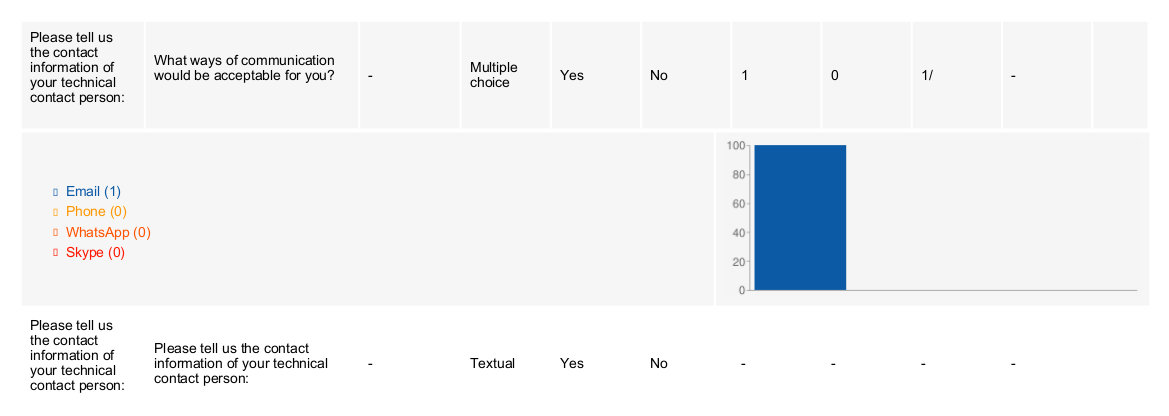
\includegraphics[width=\textwidth]{res/customerVoice/q1_results/q2.png}
%\caption{Overview of first Questionnaire's Results}
%\label{fig:resultsOverview}
\end{figure}

\begin{figure}
\centering
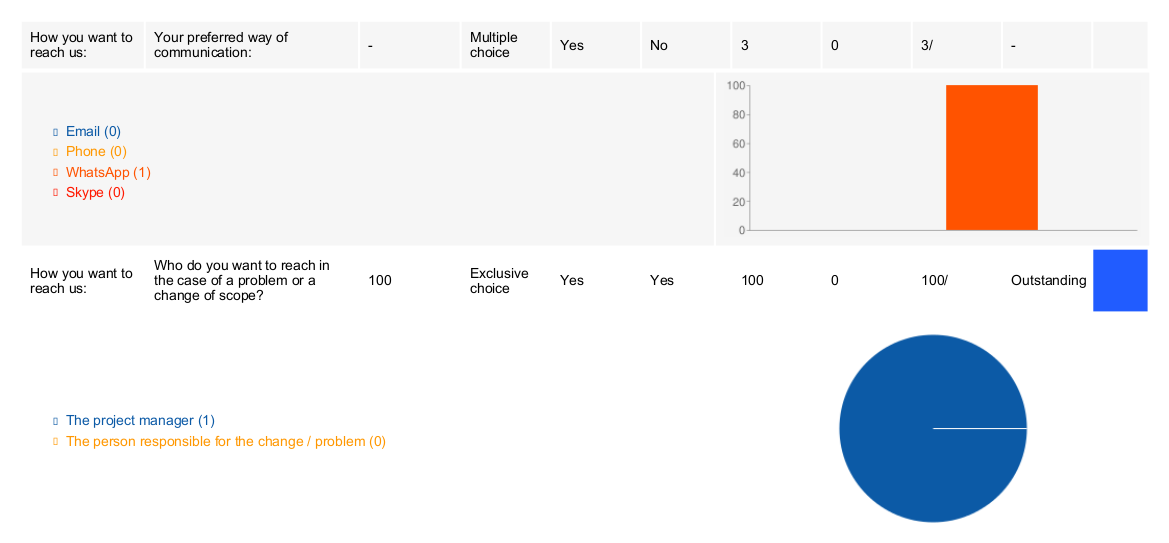
\includegraphics[width=\textwidth]{res/customerVoice/q1_results/q3.png}
%\caption{Overview of first Questionnaire's Results}
%\label{fig:resultsOverview}
\end{figure}

\begin{figure}
\centering
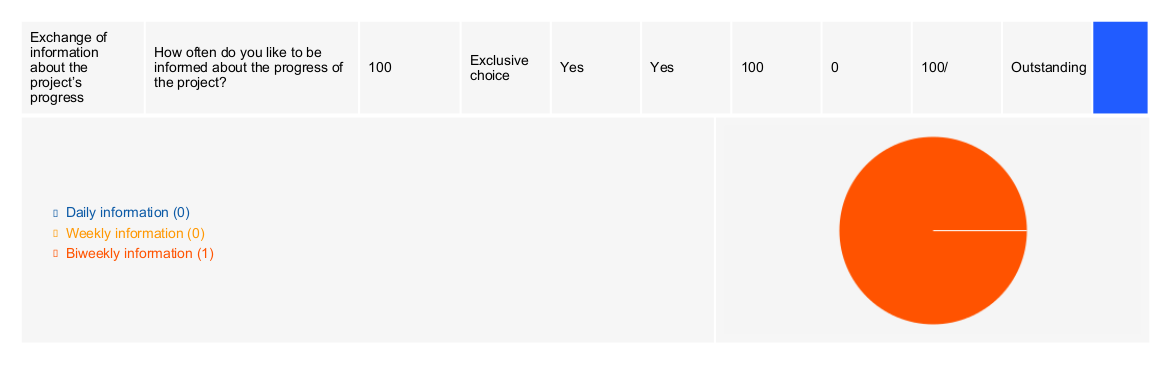
\includegraphics[width=\textwidth]{res/customerVoice/q1_results/q4.png}
%\caption{Overview of first Questionnaire's Results}
%\label{fig:resultsOverview}
\end{figure}

\begin{figure}
\centering
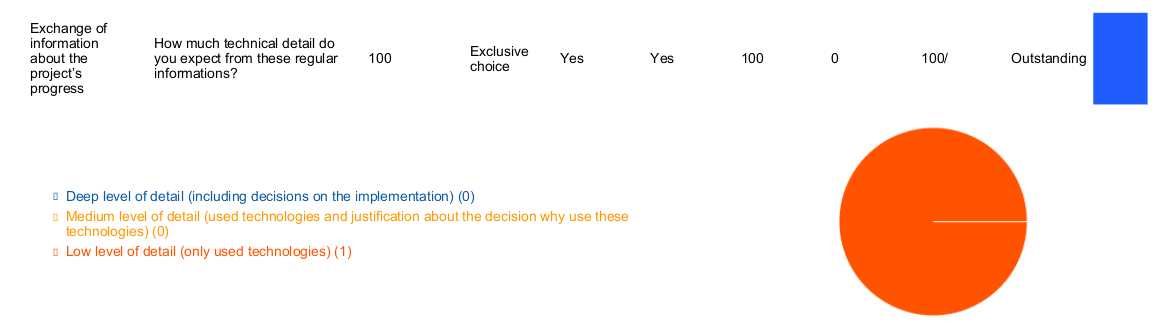
\includegraphics[width=\textwidth]{res/customerVoice/q1_results/q5.png}
%\caption{Overview of first Questionnaire's Results}
%\label{fig:resultsOverview}
\end{figure}

\begin{figure}
\centering
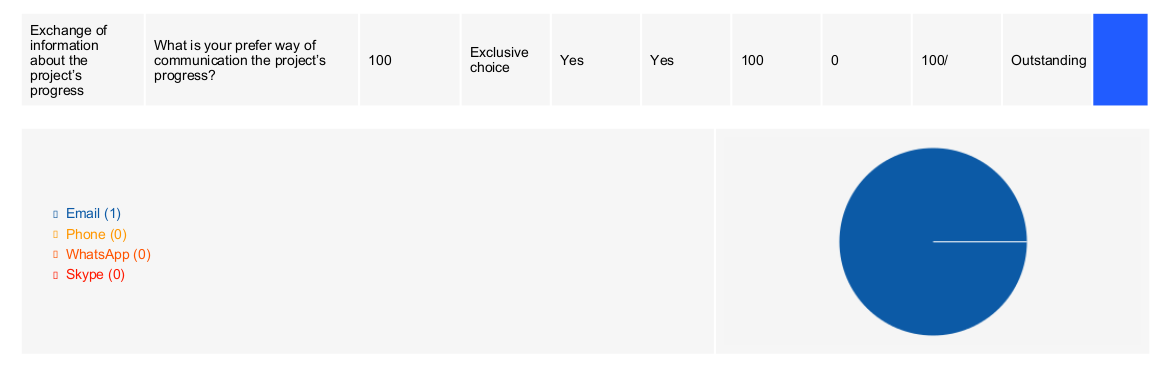
\includegraphics[width=\textwidth]{res/customerVoice/q1_results/q6.png}
%\caption{Overview of first Questionnaire's Results}
%\label{fig:resultsOverview}
\end{figure}

\begin{figure}
\centering
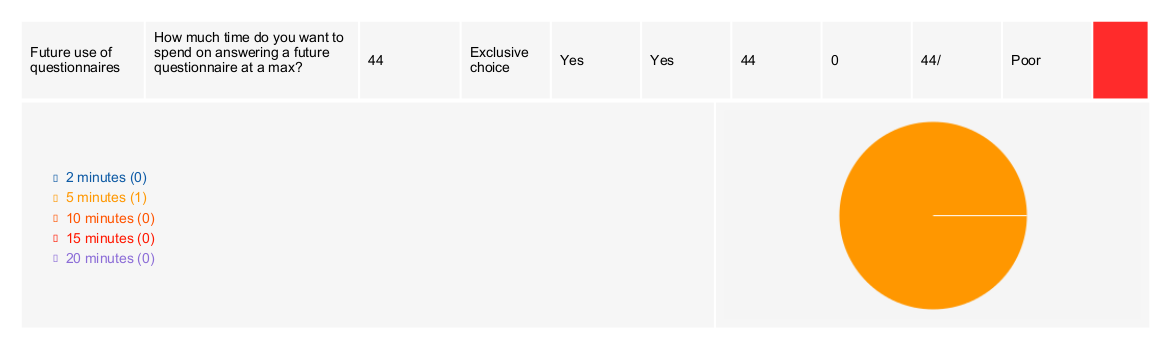
\includegraphics[width=\textwidth]{res/customerVoice/q1_results/q7.png}
%\caption{Overview of first Questionnaire's Results}
%\label{fig:resultsOverview}
\end{figure}

\begin{figure}
\centering
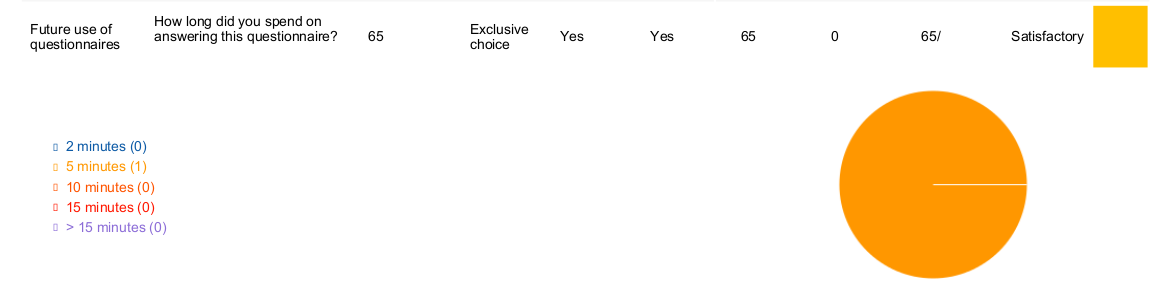
\includegraphics[width=\textwidth]{res/customerVoice/q1_results/q8.png}
%\caption{Overview of first Questionnaire's Results}
%\label{fig:resultsOverview}
\end{figure}

\begin{figure}
\centering
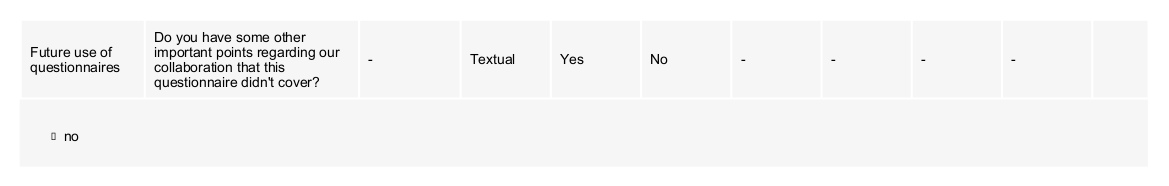
\includegraphics[width=\textwidth]{res/customerVoice/q1_results/q9.png}
%\caption{Overview of first Questionnaire's Results}
%\label{fig:resultsOverview}
\end{figure}

\FloatBarrier
\subsection{Gained Knowledge}
\label{sect:q1_results}

\begin{figure}
\centering
\captionsetup{justification=centering}
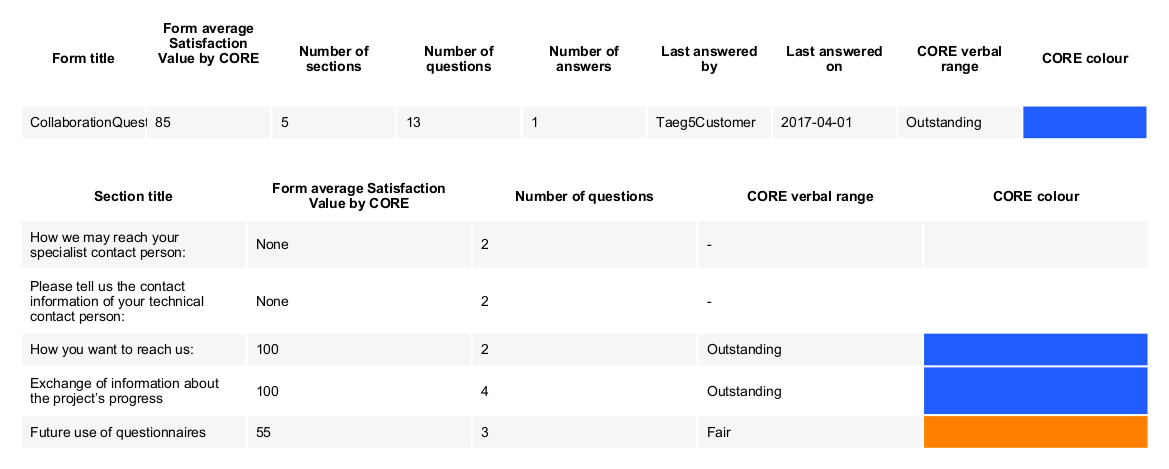
\includegraphics[width=\textwidth]{res/customerVoice/q1_results/overview.png}
\caption{Overview of first Questionnaire's Results}
\label{fig:resultsOverview}
\end{figure}

The result of the questionnaire is as well important as it is satisfactory to
our company since the most answers given by the customer reflect the preferences
of our company. This is especially true regarding the questions on the way our
company will contact the customer, on the interval that is used for reporting
and on the reporting's level of detail.

While the fact that our customer wants to contact the project manager and not
any other team member complies with our company's preferences, the way of
contacting him is suboptimal in our opinion. Nevertheless, our company will
attend the customer's wished in this point.

To be able to gain honest and serious feedback from following questionnaires and
not to overstrain our customer's willingness to collaborate, the last section
deals with questionnaires in general. It is determined how long it took to
answer the current questionnaire and how much time our customer is willing to
spent in answering future questionnaires. For the simple reason that it was
estimated that answering the current questionnaire would take 10 minutes, the
CORE value retrieved from the answers on these questions is not highest
achievable value. However, the result shows that the questionnaire's length
perfectly fit the customer's preferences. Future questionnaires will therefore
be designed in a way that they nearly have the same length and the CORE values
for the options on the question how long it took to answer a questionnaire 
will be adapted.

\section{Clarification of the Requirements and Assessment of the first Design}
Prototype Gathering and writing down requirements for a product requires high
prudence. \cite{Young} defines 15 characteristics of good requirements. Even if
high effort is expended in the process of requirements engineering, there are
mostly requirements that don't exhibit all of these characteristics. In the most
cases, these requirements lack clarity and expressiveness.

The unclear requirements as well as a first mockup are the basis of a second
questionnaire. Its aims are to inform the customer how the vague requirements
were interpreted in the first step, to offer the customer the possibility to
give a feedback on this interpretation and to provide him a first sense of the
product that will be developed. The mockup that was created for the purpose of
this questionnaire is depicted in figure \ref{fig:initialMockup}.

\begin{figure}
\centering
\captionsetup{justification=centering}
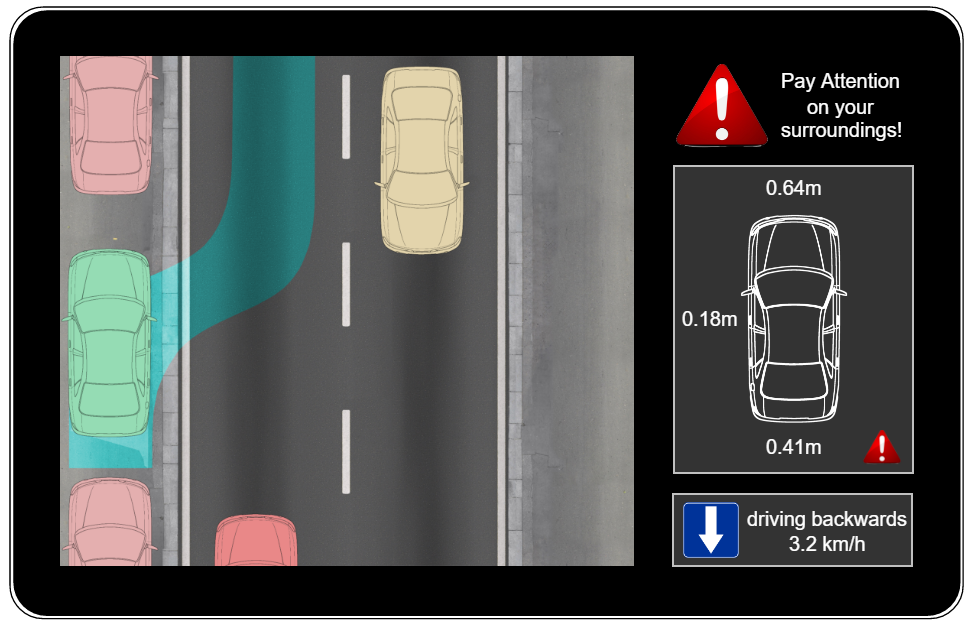
\includegraphics[width=0.75\textwidth]{res/customerVoice/mockup.png}
\caption{Initial Mockup of the System}
\label{fig:initialMockup}
\end{figure}

\subsection{Results}
The results that help to clarify the requirements and to get a first feedback on
the planned design are depicted below and interpreted in the next section (see
section \ref{sect:q2_results}). Since a mistake has been made on the creation of
the questionnaire, the assessment how long it took the customer to answer it had
to be done in an additional form. The results of the initial survey and the
additional form are assembled together.

\begin{figure}[h!]
\centering
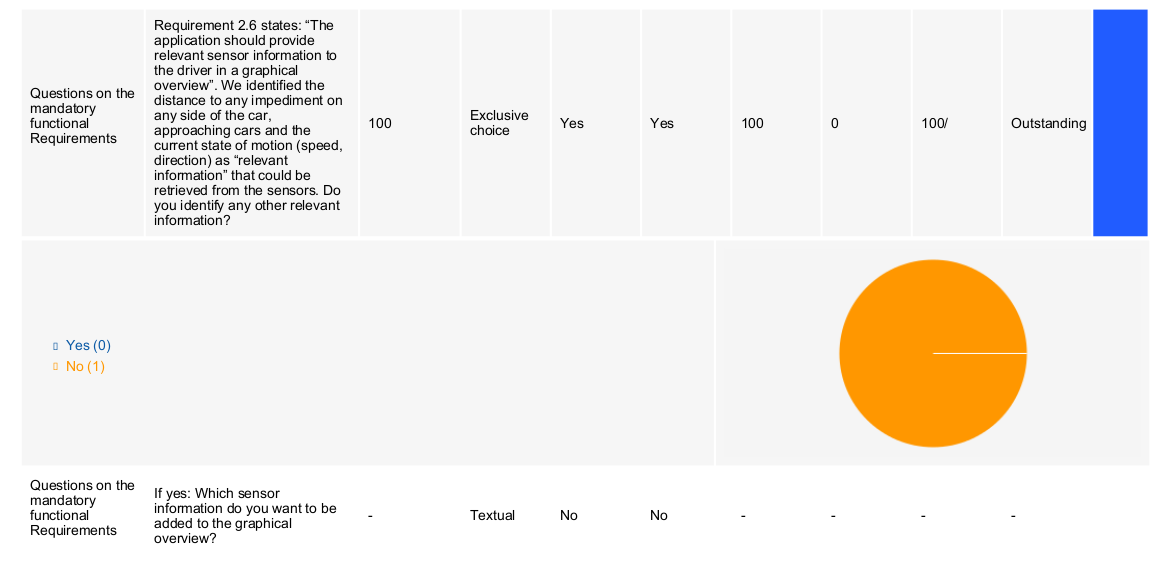
\includegraphics[width=\textwidth]{res/customerVoice/q2_results/q1.png}
%\caption{Overview of first Questionnaire's Results}
%\label{fig:resultsOverview}
\end{figure}

\begin{figure}
\centering
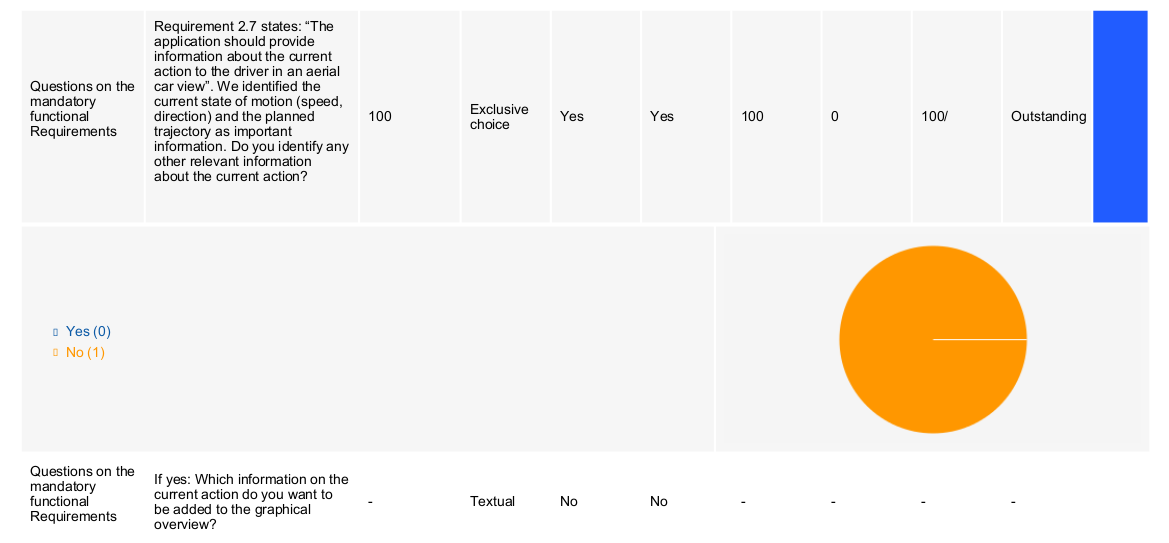
\includegraphics[width=\textwidth]{res/customerVoice/q2_results/q2.png}
%\caption{Overview of first Questionnaire's Results}
%\label{fig:resultsOverview}
\end{figure}

\begin{figure}
\centering
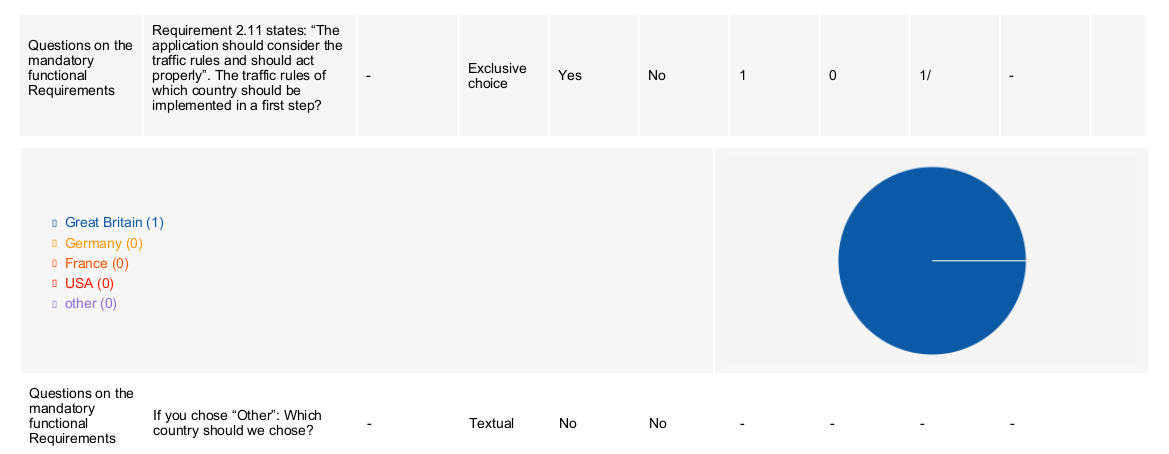
\includegraphics[width=\textwidth]{res/customerVoice/q2_results/q3.png}
%\caption{Overview of first Questionnaire's Results}
%\label{fig:resultsOverview}
\end{figure}

\begin{figure}
\centering
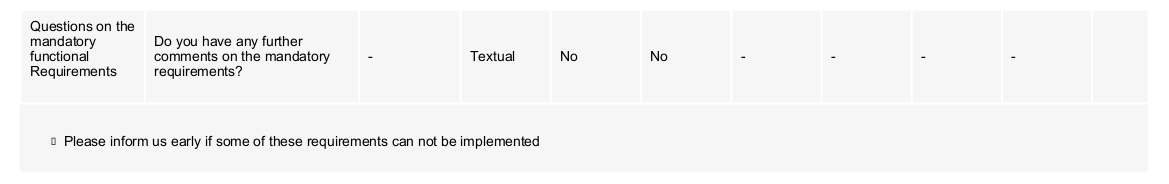
\includegraphics[width=\textwidth]{res/customerVoice/q2_results/q4.png}
%\caption{Overview of first Questionnaire's Results}
%\label{fig:resultsOverview}
\end{figure}

\begin{figure}
\centering
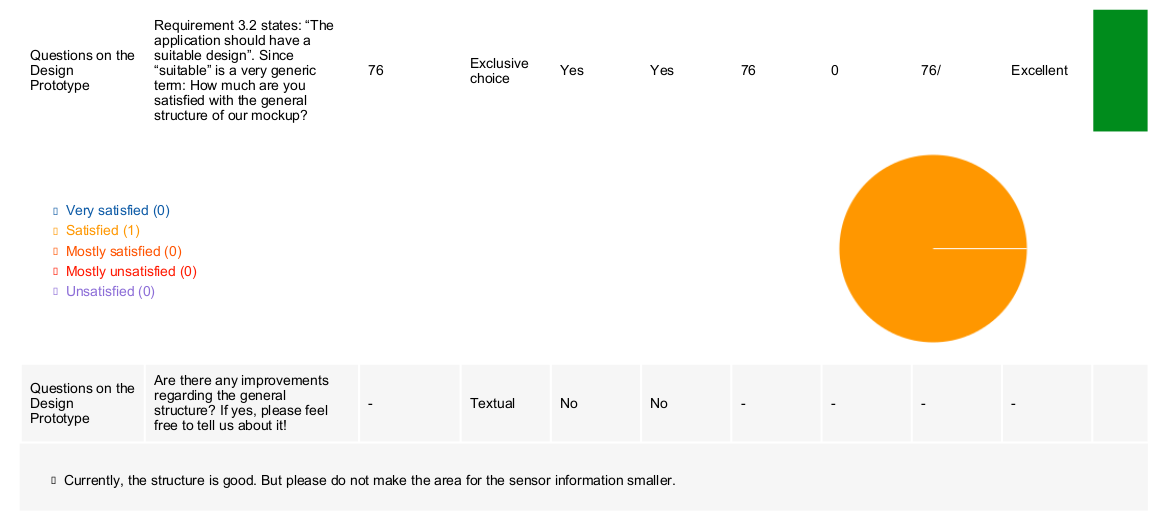
\includegraphics[width=\textwidth]{res/customerVoice/q2_results/q5.png}
%\caption{Overview of first Questionnaire's Results}
%\label{fig:resultsOverview}
\end{figure}

\begin{figure}
\centering
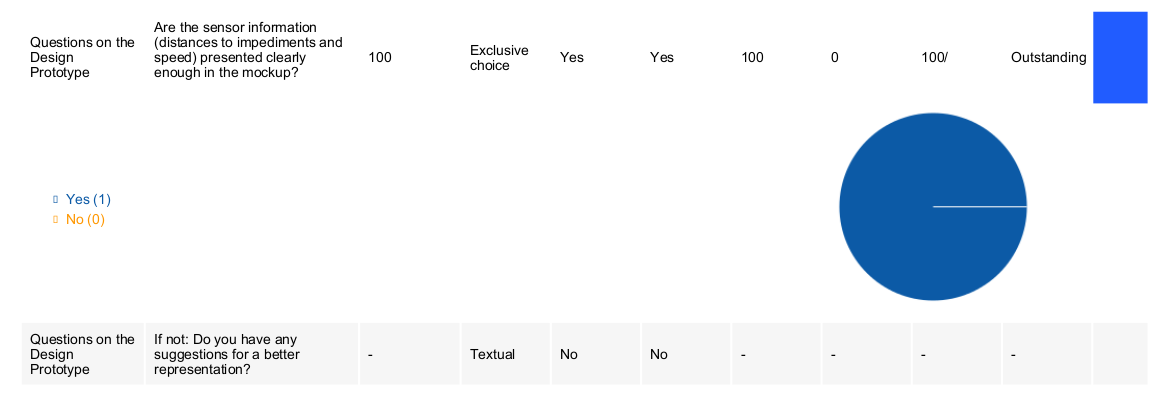
\includegraphics[width=\textwidth]{res/customerVoice/q2_results/q6.png}
%\caption{Overview of first Questionnaire's Results}
%\label{fig:resultsOverview}
\end{figure}

\begin{figure}
\centering
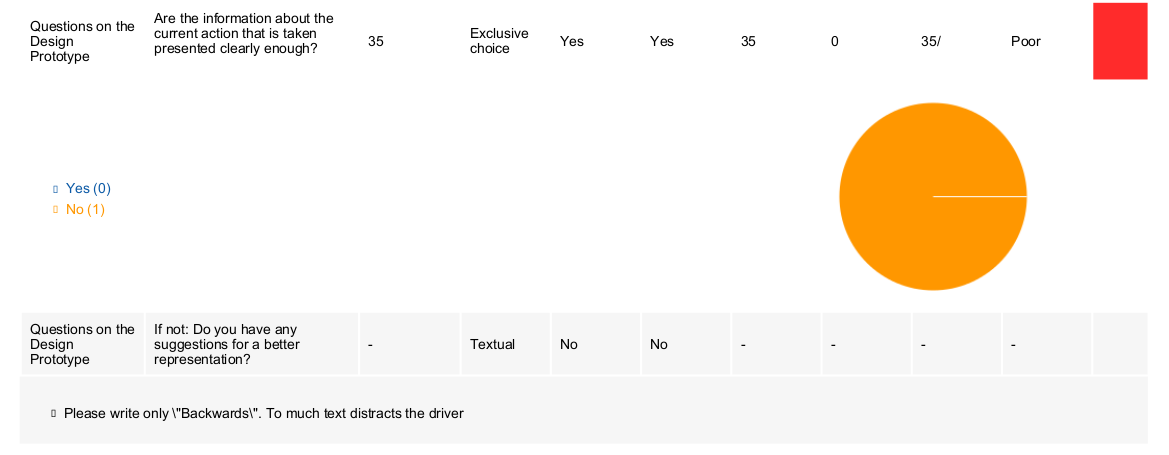
\includegraphics[width=\textwidth]{res/customerVoice/q2_results/q7.png}
%\caption{Overview of first Questionnaire's Results}
%\label{fig:resultsOverview}
\end{figure}

\begin{figure}
\centering
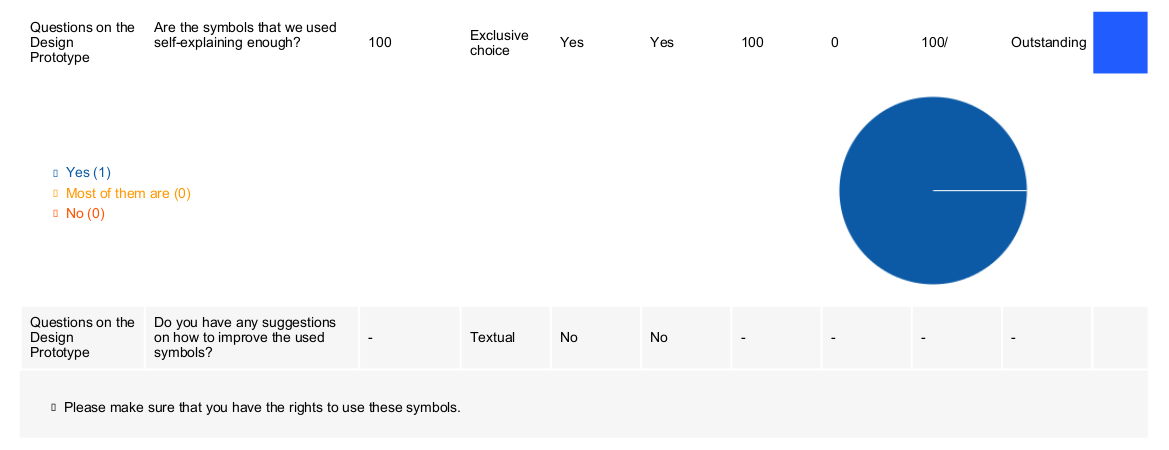
\includegraphics[width=\textwidth]{res/customerVoice/q2_results/q8.png}
%\caption{Overview of first Questionnaire's Results}
%\label{fig:resultsOverview}
\end{figure}

\begin{figure}
\centering
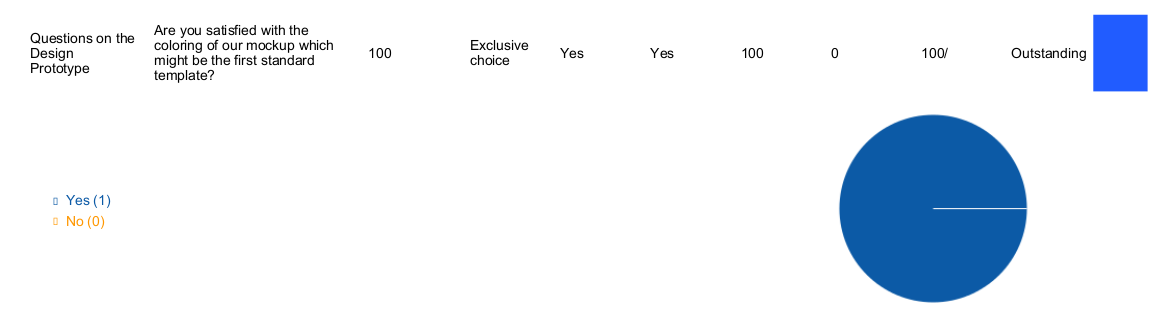
\includegraphics[width=\textwidth]{res/customerVoice/q2_results/q9.png}
%\caption{Overview of first Questionnaire's Results} 
%\label{fig:resultsOverview}
\end{figure}

\begin{figure}
\centering
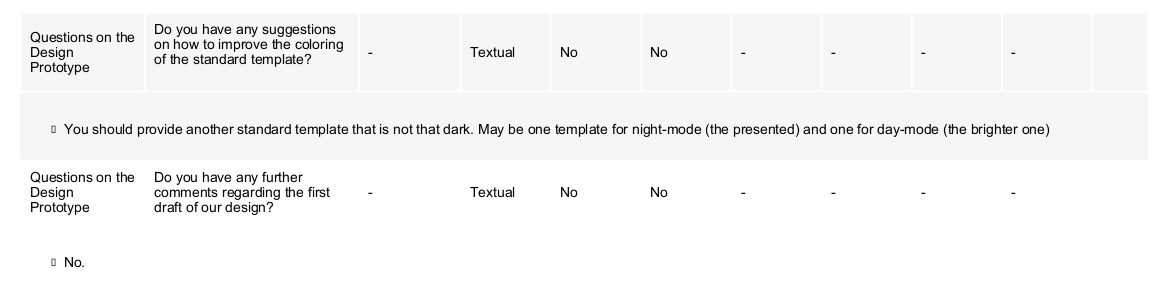
\includegraphics[width=\textwidth]{res/customerVoice/q2_results/q10.png}
%\caption{Overview of first Questionnaire's Results}
%\label{fig:resultsOverview}
\end{figure}

\begin{figure}
\centering
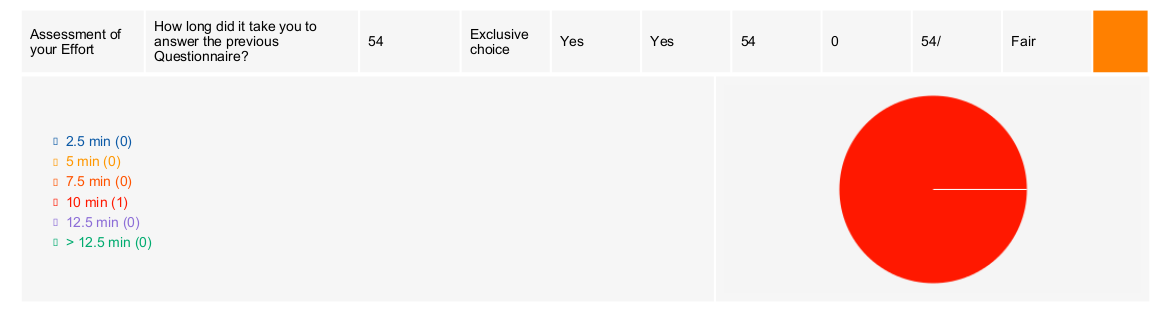
\includegraphics[width=\textwidth]{res/customerVoice/q2_results/q11.png}
%\caption{Overview of first Questionnaire's Results}
%\label{fig:resultsOverview}
\end{figure}

\FloatBarrier

\subsection{Gained Knowledge and further Steps taken}
\label{sect:q2_results}

\begin{figure}
\centering
\captionsetup{justification=centering}
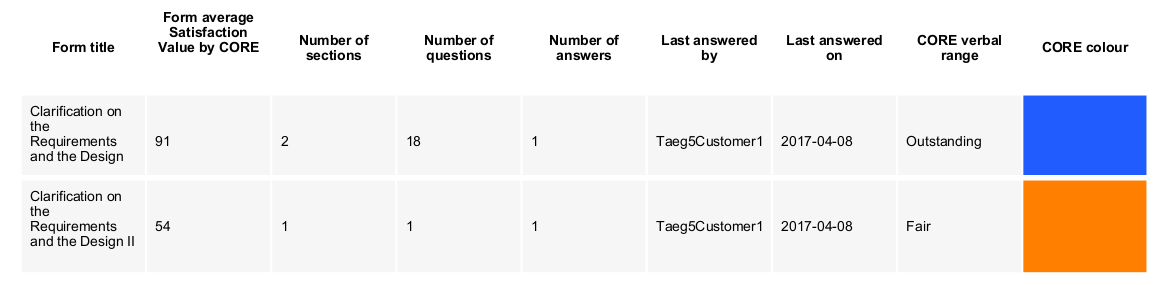
\includegraphics[width=\textwidth]{res/customerVoice/q2_results/overview.png}
\caption{Overview of second Questionnaire's Results}
\label{fig:resultsOverview2}
\end{figure}

As it can be seen in \ref{fig:resultsOverview2}, the results are very satisfying
and the interpretation of the requirements fits the customer's expectations.
More detailed feedback could be gathered regarding the design of the system. In
the further development, our company will focus its attention to simplify the
design e.g. by shortening the presented texts and by trying to scale up the area
that presents the sensor information.

Unfortunately, the customer was not able to answer the questionnaire within 5
minutes as preferred, although the open questions on the optional requirements
were already omitted. Since this was expected and the clarification of the
requirements is a very important point, it is acceptable in the case of the
current survey. Nevertheless, there has to be some effort made in the future to
keep the questionnaires as short as possible for not deceiving the customer
again in this regard.

\section{Interim Report about the Project's Progress}
As it was determined in the first questionnaire (see section 
\ref{sect:firstQuestionnaire}), our customer wishes to get biweekly information
about the project's current progress. The information included should exhibit a
low level of technical detail and only reflect the relevant design decisions. A
sample report can be found in the following pages.

\FloatBarrier

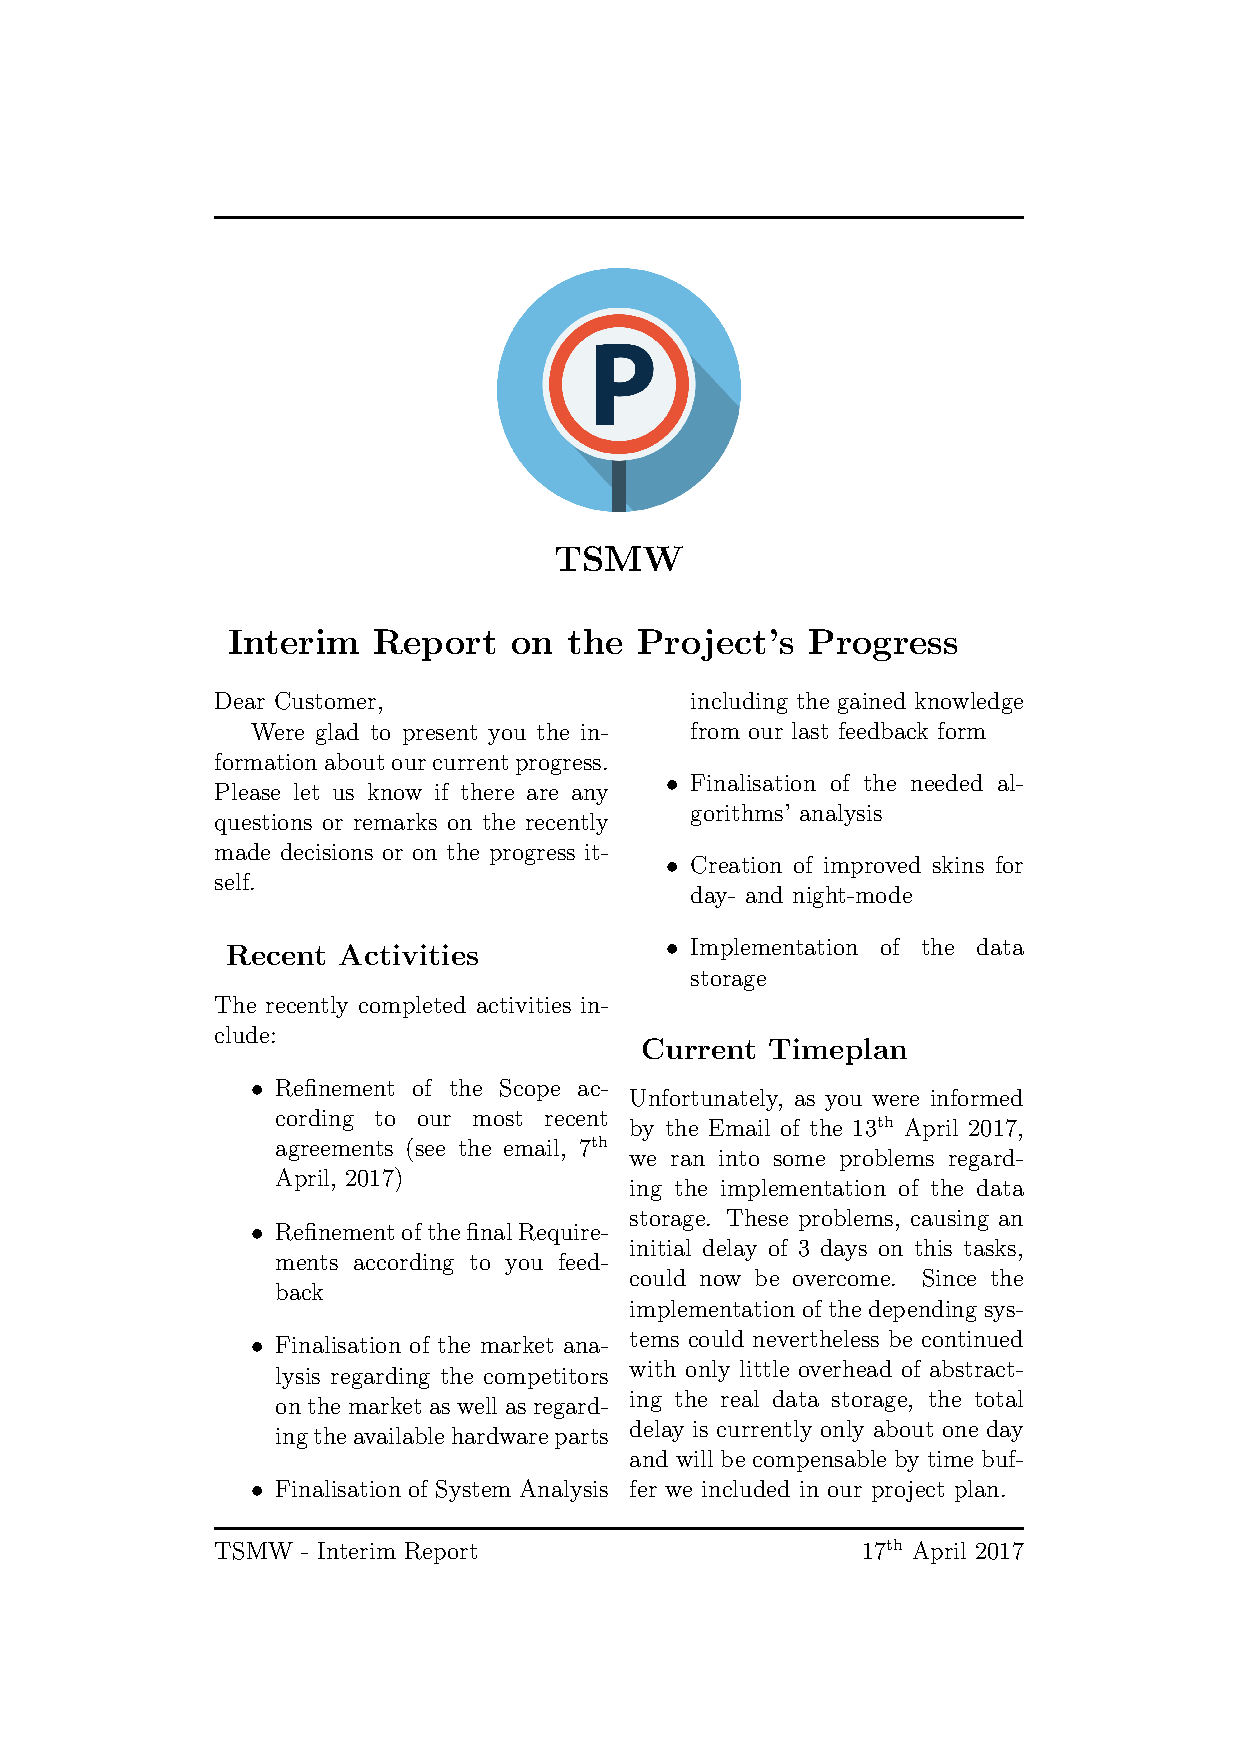
\includepdf[pages={-}]{res/customerVoice/interimReport/interimReport.pdf}

\section{Final Evaluation of the customers satisfaction}
Up to this point, Satistica was mainly used to clarify open questions. After the
termination of the project, it is important to determine the customer's
satisfaction to be able to perform better in subsequent projects. The main
points that are examined in the questionnaire are:

\begin{itemize}
\item{The customer�s satisfaction with our communication}
\item{The customer�s satisfaction with the process of gathering and implementing its feedback}
\item{The customer�s satisfaction with the reports provided}
\end{itemize}

\subsection{Results}
The single question's results are again depicted in the current section. The
summary of the overall feedback form is depicted in section
\ref{sect:q3_results}.

\begin{figure}[h!]
\centering
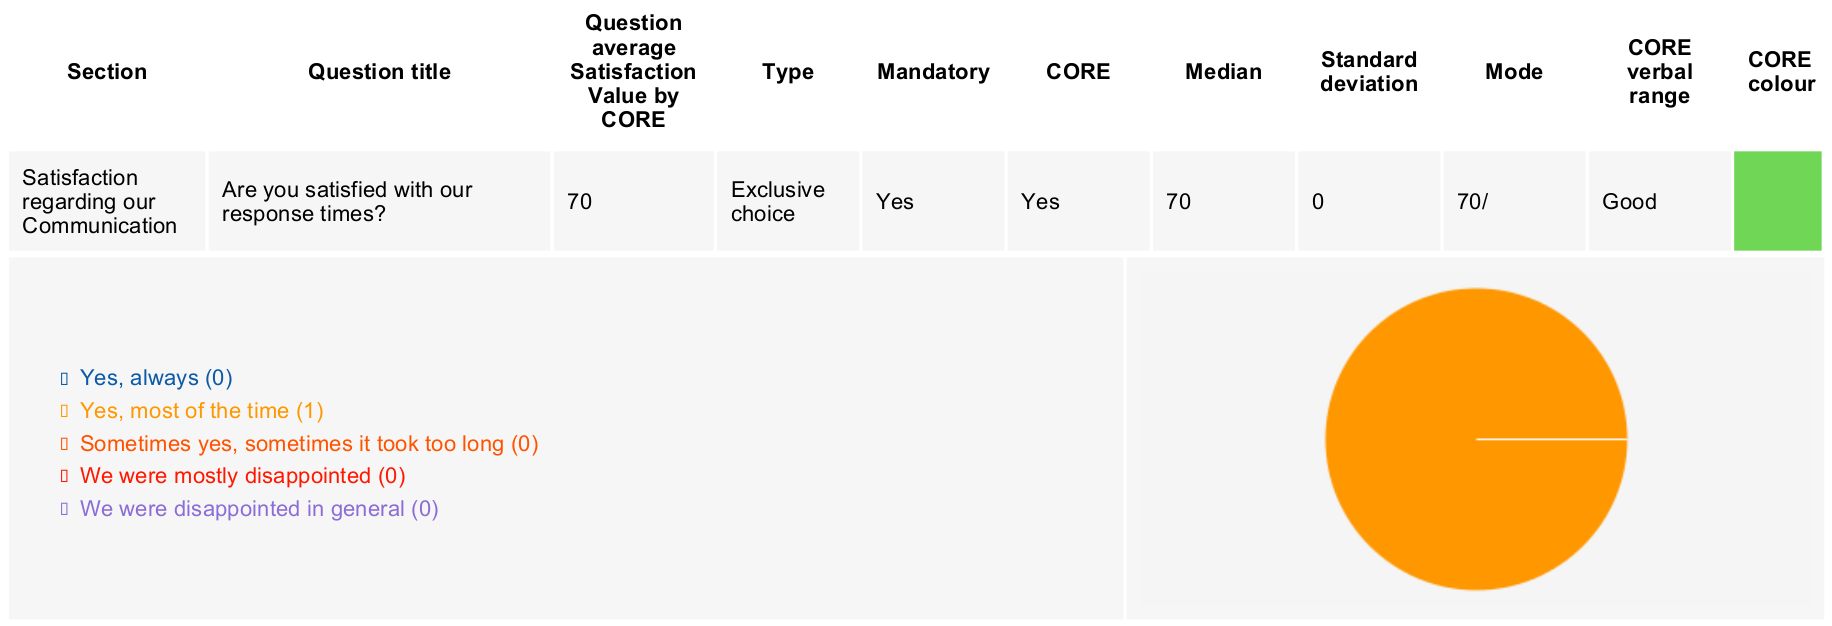
\includegraphics[width=\textwidth]{res/customerVoice/q3_results/q1.png}
%\caption{Overview of first Questionnaire's Results}
%\label{fig:resultsOverview}
\end{figure}

\begin{figure}
\centering
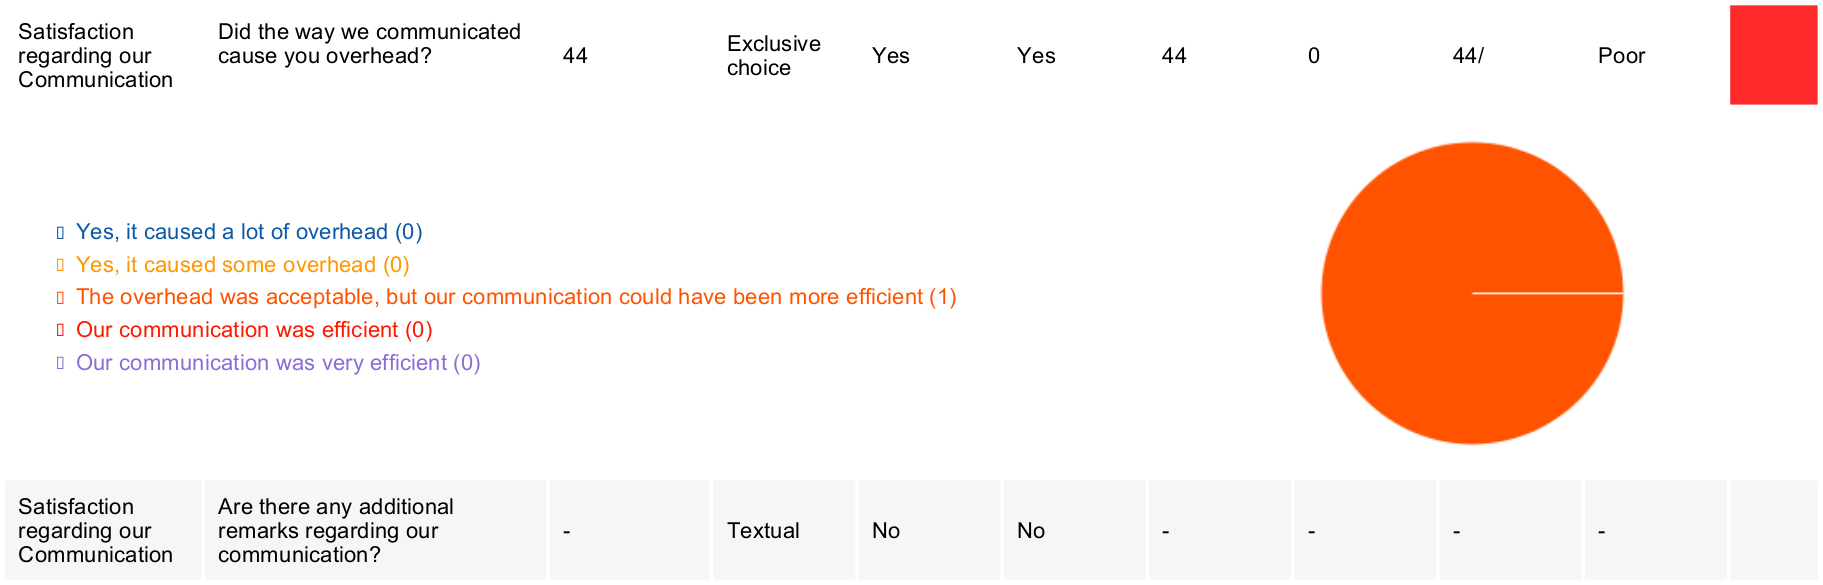
\includegraphics[width=\textwidth]{res/customerVoice/q3_results/q2.png}
%\caption{Overview of first Questionnaire's Results}
%\label{fig:resultsOverview}
\end{figure}

\begin{figure}
\centering
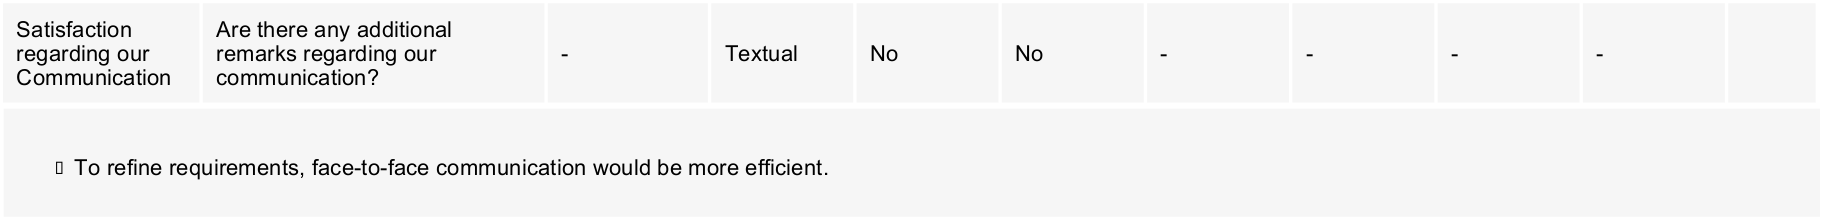
\includegraphics[width=\textwidth]{res/customerVoice/q3_results/q3.png}
%\caption{Overview of first Questionnaire's Results}
%\label{fig:resultsOverview}
\end{figure}

\begin{figure}
\centering
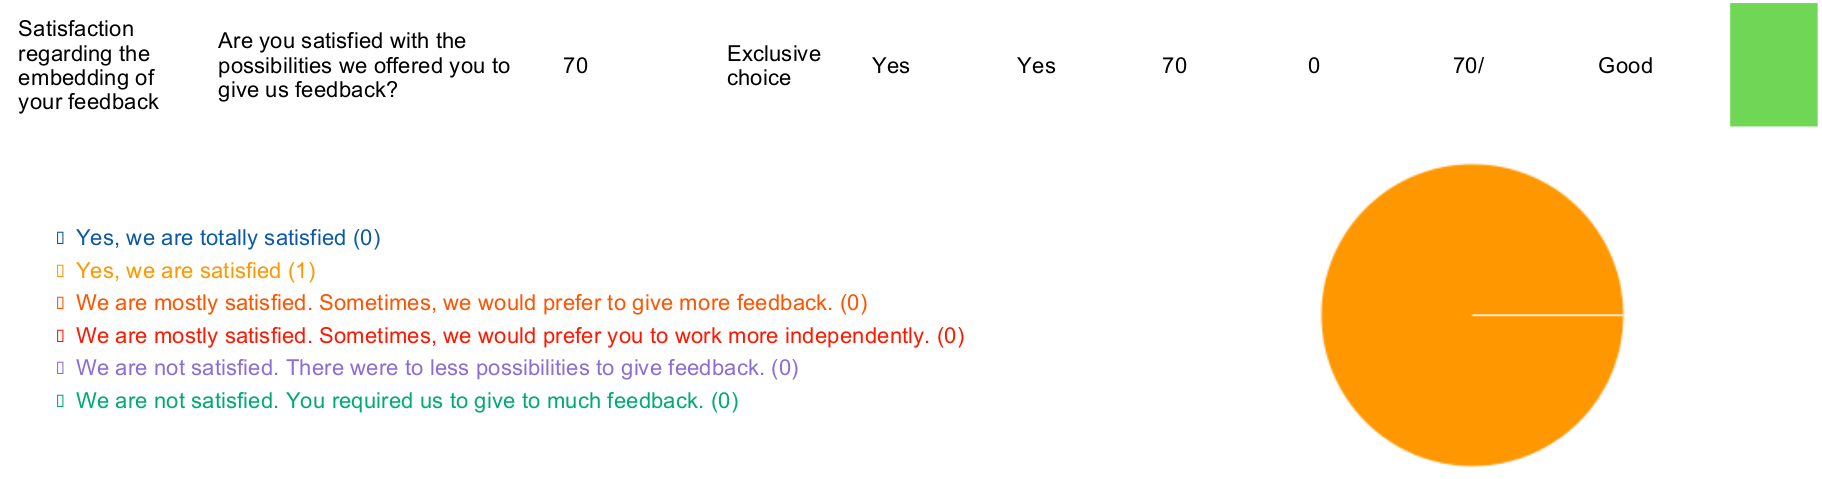
\includegraphics[width=\textwidth]{res/customerVoice/q3_results/q4.png}
%\caption{Overview of first Questionnaire's Results}
%\label{fig:resultsOverview}
\end{figure}

\begin{figure}
\centering
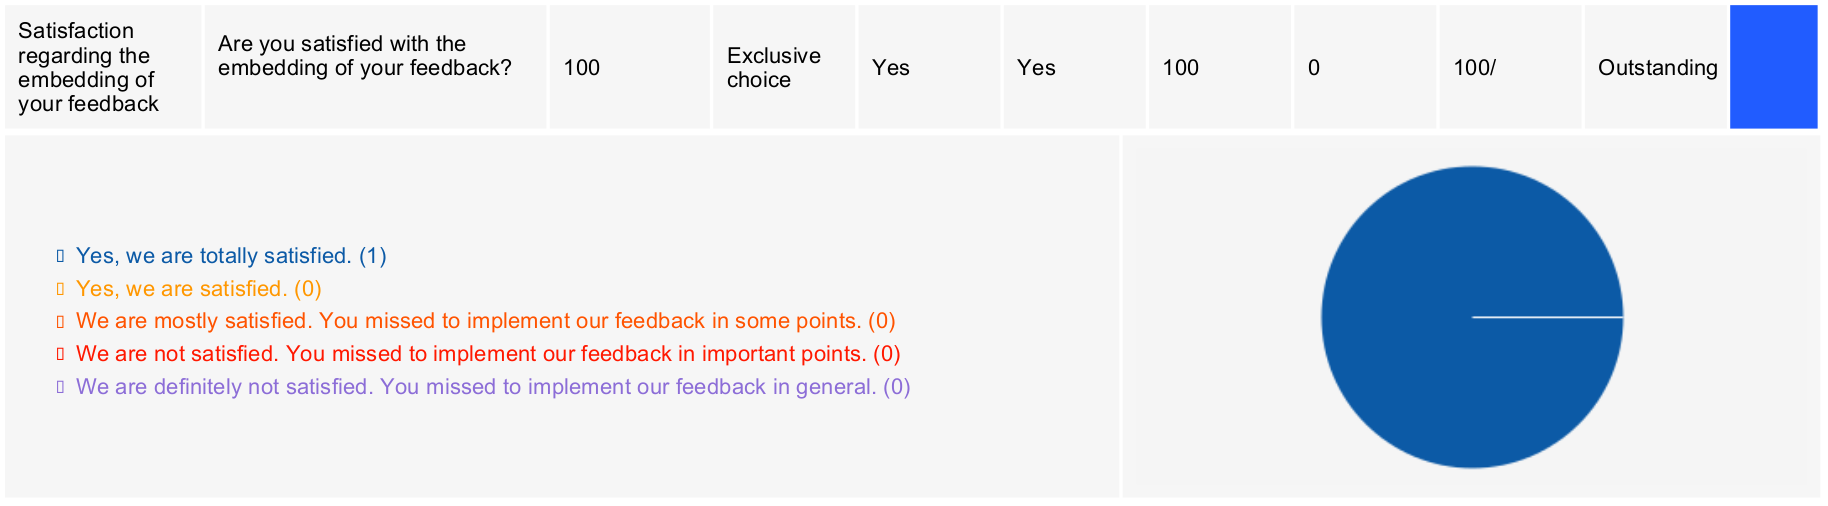
\includegraphics[width=\textwidth]{res/customerVoice/q3_results/q5.png}
%\caption{Overview of first Questionnaire's Results}
%\label{fig:resultsOverview}
\end{figure}

\begin{figure}
\centering
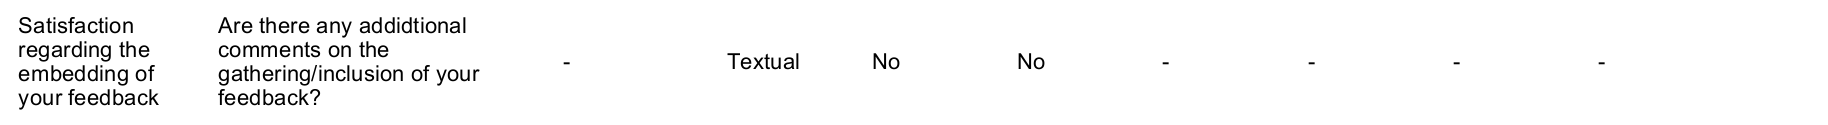
\includegraphics[width=\textwidth]{res/customerVoice/q3_results/q6.png}
%\caption{Overview of first Questionnaire's Results}
%\label{fig:resultsOverview}
\end{figure}

\begin{figure}
\centering
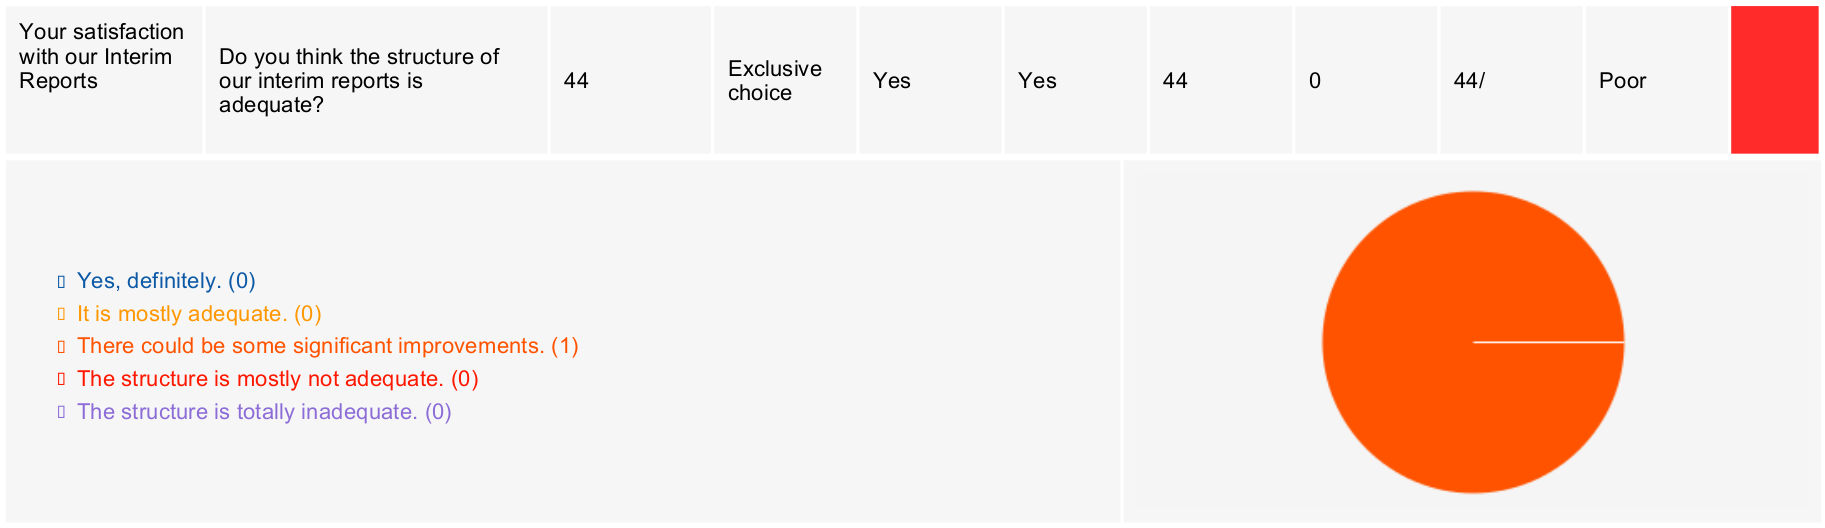
\includegraphics[width=\textwidth]{res/customerVoice/q3_results/q7.png}
%\caption{Overview of first Questionnaire's Results}
%\label{fig:resultsOverview}
\end{figure}

\begin{figure}
\centering
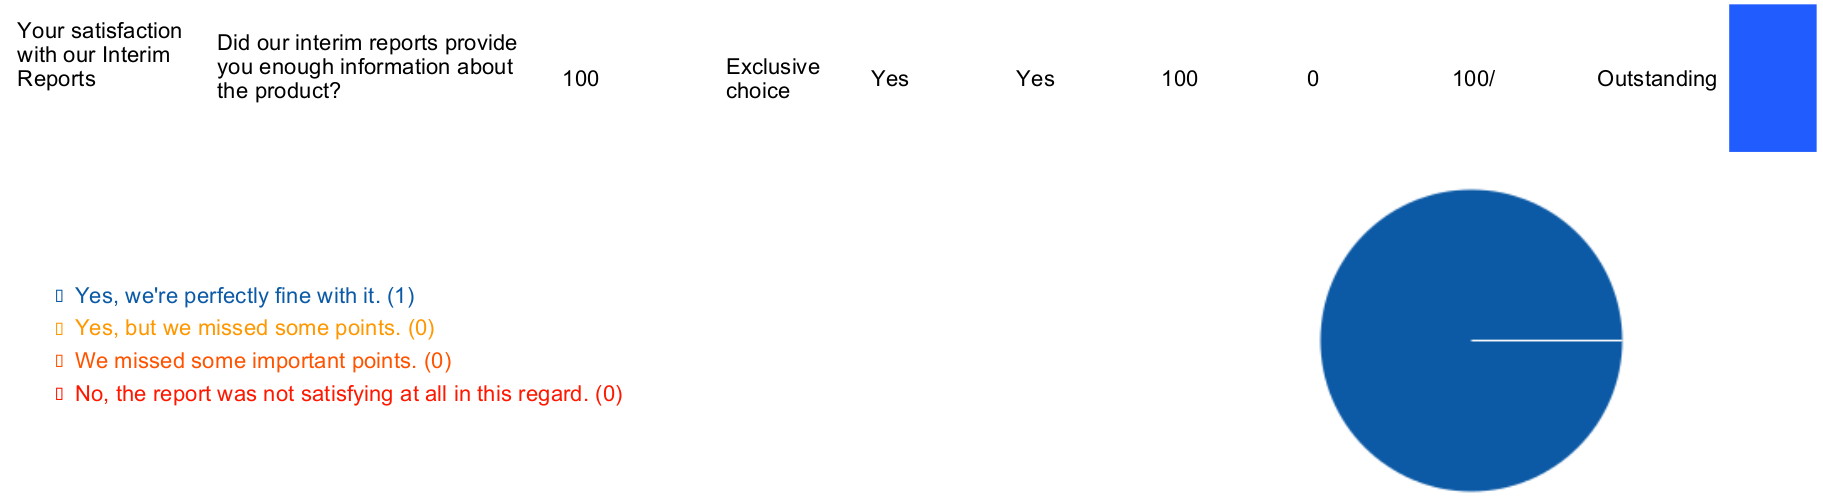
\includegraphics[width=\textwidth]{res/customerVoice/q3_results/q8.png}
%\caption{Overview of first Questionnaire's Results}
%\label{fig:resultsOverview}
\end{figure}

\begin{figure}
\centering
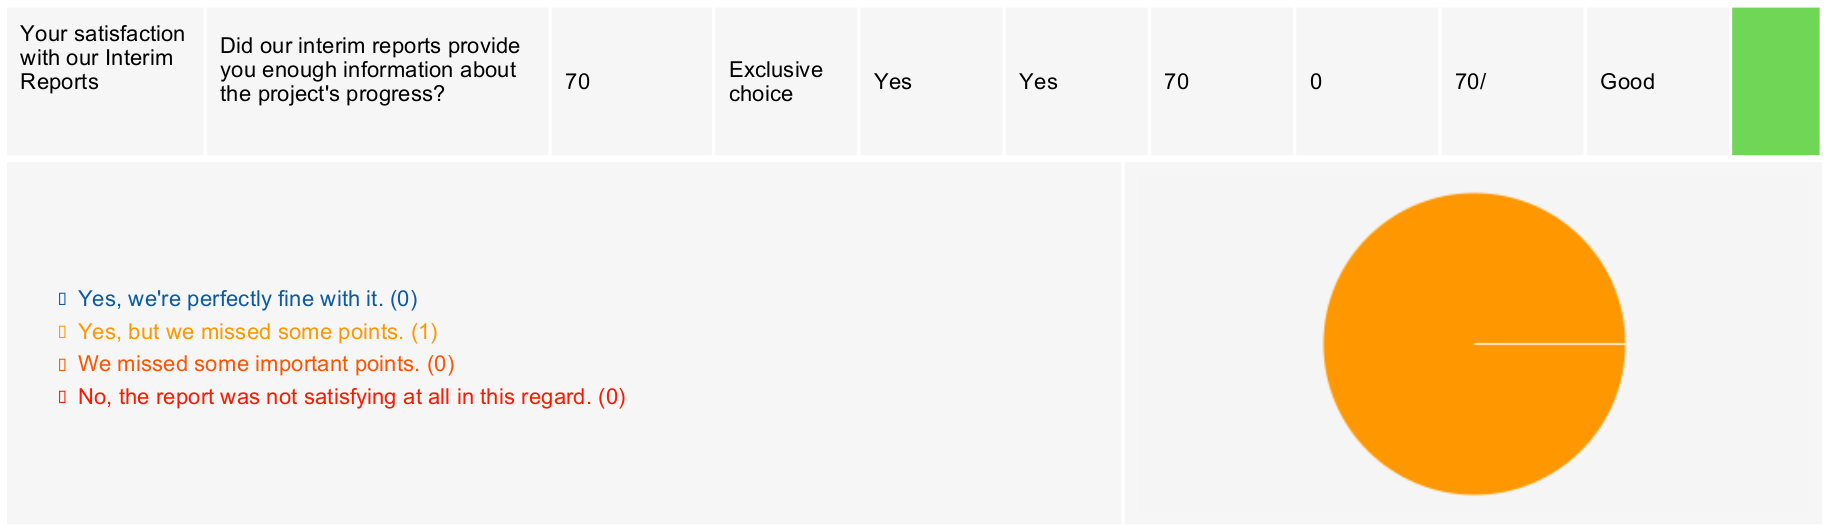
\includegraphics[width=\textwidth]{res/customerVoice/q3_results/q9.png}
%\caption{Overview of first Questionnaire's Results} 
%\label{fig:resultsOverview}
\end{figure}

\begin{figure}
\centering
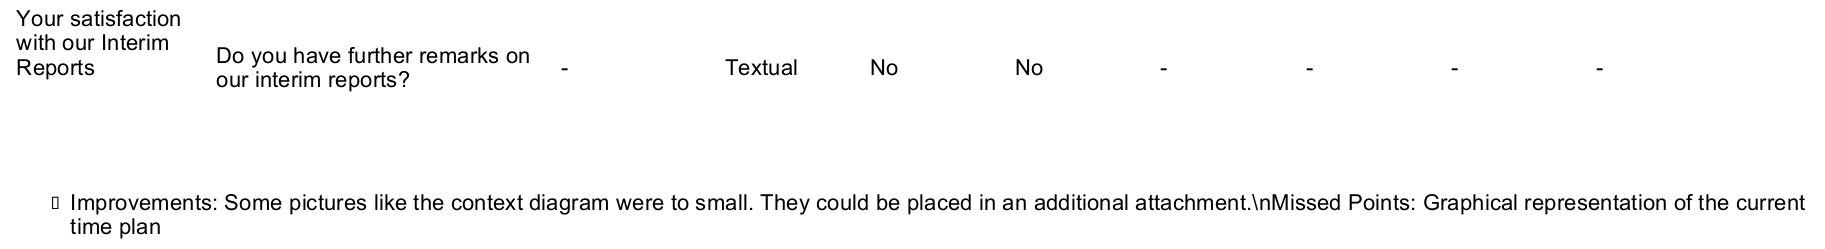
\includegraphics[width=\textwidth]{res/customerVoice/q3_results/q10.png}
%\caption{Overview of first Questionnaire's Results}
%\label{fig:resultsOverview}
\end{figure}

\begin{figure}
\centering
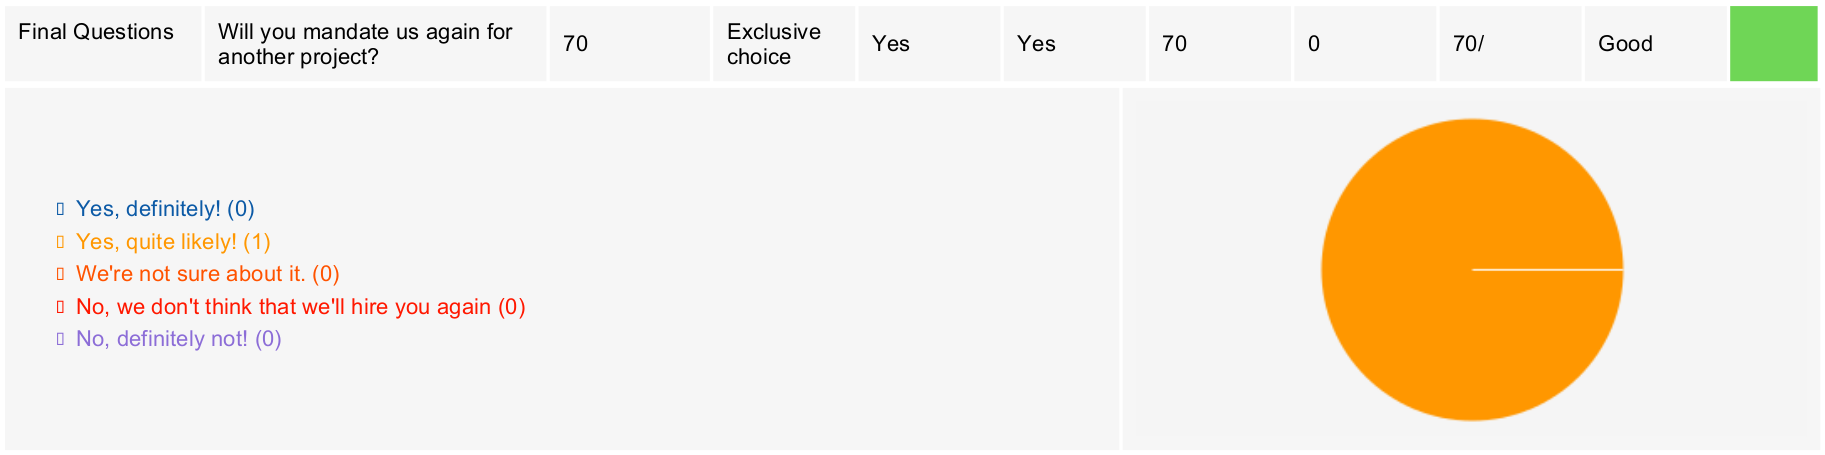
\includegraphics[width=\textwidth]{res/customerVoice/q3_results/q11.png}
%\caption{Overview of first Questionnaire's Results}
%\label{fig:resultsOverview}
\end{figure}

\begin{figure}
\centering
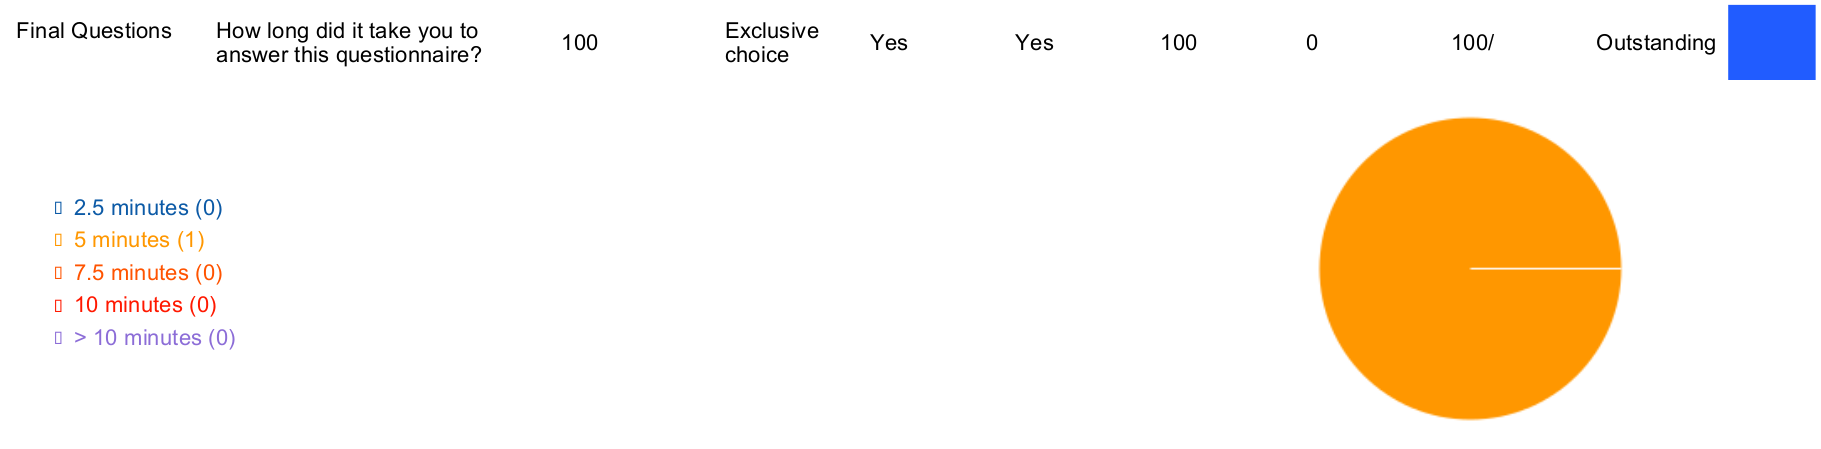
\includegraphics[width=\textwidth]{res/customerVoice/q3_results/q12.png}
%\caption{Overview of first Questionnaire's Results}
%\label{fig:resultsOverview}
\end{figure}

\FloatBarrier

\subsection{Gained Knowledge}
\label{sect:q3_results}

The knowledge that could be extracted from the last questionnaire cannot be
applied to the current project since the questionnaire. Nevertheless, the gained
knowledge is very important in regard to the aim of continuous improvement of
our company and can be applied to subsequen projects.

One of the questionnaires outcomes is that the interim reports should be
improved. The two-columns-layout implicates the problem of pictures being two
small. In some points, e.g. if the progress of the project is stated, textual
descriptions might be avoided by using expressive charts.

In addition, our company will cherish the idea of face-to-face communication
being the most efficient way of clarifying open questions. The overall result of
the last feedback form is depicted in figure \ref{fig:resultsOverview3}.


\begin{figure}[h!]
\centering
\captionsetup{justification=centering}
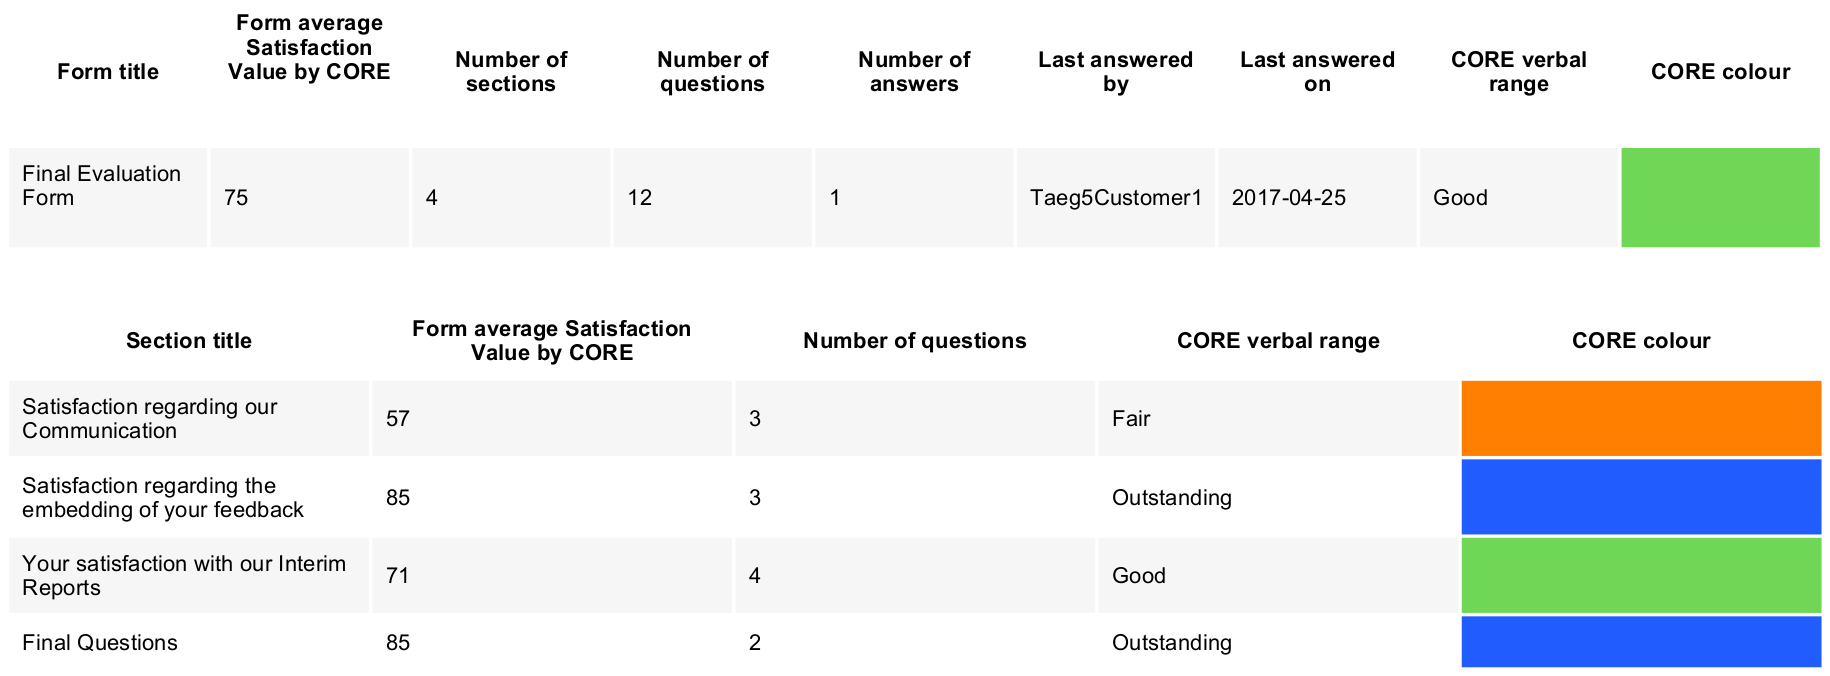
\includegraphics[width=\textwidth]{res/customerVoice/q3_results/overview.png}
\caption{Overview of second Questionnaire's Results}
\label{fig:resultsOverview3}
\end{figure}